%-----------------------------------LICENSE------------------------------------%
%   This file is part of tikz_figures.                                         %
%                                                                              %
%   tikz_figures is free software: you can redistribute it and/or              %
%   modify it it under the terms of the GNU General Public License as          %
%   published by the Free Software Foundation, either version 3 of the         %
%   License, or (at your option) any later version.                            %
%                                                                              %
%   tikz_figures is distributed in the hope that it will be useful,            %
%   but WITHOUT ANY WARRANTY; without even the implied warranty of             %
%   MERCHANTABILITY or FITNESS FOR A PARTICULAR PURPOSE.  See the              %
%   GNU General Public License for more details.                               %
%                                                                              %
%   You should have received a copy of the GNU General Public License along    %
%   with tikz_figures.  If not, see <https://www.gnu.org/licenses/>.           %
%------------------------------------------------------------------------------%

% Use the standalone class for displaying the tikz image on a small PDF.
\documentclass[crop, tikz]{standalone}

% Import the tikz package to use for the drawing.
\usepackage{tikz}

% tikz libraries used in the drawing.
\usetikzlibrary{
    angles, % Drawing angles within triangles.
    quotes, % Adding labels to angles.
}

% Begin the document.
\begin{document}

    % Draw the figure.
    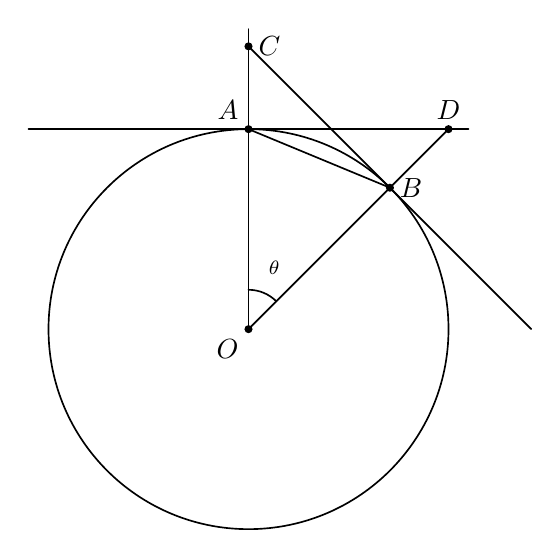
\begin{tikzpicture}[%
        line width = 0.6pt,
        line cap = round
    ]

        % Nodes for all of the points.
        \coordinate (O) at (0, 0);
        \coordinate (A) at (0, 1in);
        \coordinate (B) at (0.7071in, 0.7071in);
        \coordinate (C) at (0, 1.414in);
        \coordinate (D) at (1in, 1in);
        \coordinate (E) at (1.414in, 0);

        % Draw in the lines and circles for the figure.
        \draw (O) circle (1in);
        \draw (-1.1in, 1in) to (1.1in, 1in);
        \draw (O) to (0, 1.5in);
        \draw (A) to (B);
        \draw (O) to (D);
        \draw (C) to (E);

        % Label points with dots.
        \draw[fill = black] (O) circle (0.4mm);
        \draw[fill = black] (A) circle (0.4mm);
        \draw[fill = black] (B) circle (0.4mm);
        \draw[fill = black] (C) circle (0.4mm);
        \draw[fill = black] (D) circle (0.4mm);

        % Label all of the nodes.
        \node at (O) [below left] {$O$};
        \node at (A) [above left] {$A$};
        \node at (B) [right] {$B$};
        \node at (C) [right] {$C$};
        \node at (D) [above] {$D$};

        % Draw in an arc for the angle theta.
        \pic[%
            draw = black,
            "\scriptsize{${\theta}$}",
            angle eccentricity = 1.7,
            angle radius = 0.5cm
        ] {angle = D--O--C};
    \end{tikzpicture}
\end{document}
